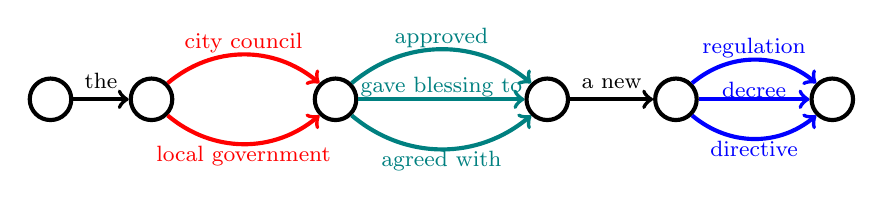
\begin{tikzpicture}	
	\tikzstyle{unit} = [circle,line width=1.5pt,draw,minimum size=1.5em]
		
		\node[unit] (u1)at (0,0){};
		\node[unit,anchor=west](u2) at ([xshift=2em]u1.east){};
		\node[unit,anchor=west](u3) at ([xshift=5em]u2.east){};
		\node[unit,anchor=west](u4) at ([xshift=6em]u3.east){};
		\node[unit,anchor=west](u5) at ([xshift=3em]u4.east){};
		\node[unit,anchor=west](u6) at ([xshift=4em]u5.east){};
		
		\draw[->,line width=1.5pt](u1.east) -- node[above]{\footnotesize the} (u2.west);
		\draw[->,out=40,in=140,red,line width=1.5pt] (u2.north east) to  node[inner sep=0pt,color=red,above]{\footnotesize city council}(u3.north west);
		\draw[->,out=-40,in=-140,red,line width=1.5pt] (u2.south east) to  node[inner sep=0pt,color=red,below]{\footnotesize local government}(u3.south west);
		
		\draw[->,out=40,in=140,teal,line width=1.5pt] (u3.north east) to  node[inner sep=0pt,color=teal,above]{\footnotesize approved}(u4.north west);
		\draw[->,teal,line width=1.5pt](u3.east)-- node[inner sep=0pt,color=teal,above]{\footnotesize gave blessing to}(u4.west);
		\draw[->,out=-40,in=-140,teal,line width=1.5pt] (u3.south east) to  node[inner sep=0pt,color=teal,below]{\footnotesize agreed with}(u4.south west);
		\draw[->,line width=1.5pt](u4.east) -- node[above]{\footnotesize a new} (u5.west);
		
		\draw[->,out=40,in=140,blue,line width=1.5pt] (u5.north east) to  node[inner sep=0pt,color=blue,above]{\footnotesize regulation}(u6.north west);
		\draw[->,blue,line width=1.5pt](u5.east)-- node[inner sep=0pt,color=blue,above]{\footnotesize decree}(u6.west);
		\draw[->,out=-40,in=-140,blue,line width=1.5pt] (u5.south east) to  node[inner sep=0pt,color=blue,below]{\footnotesize directive}(u6.south west);
		
\end{tikzpicture}
